\documentclass[12pt,a4paper]{article}

% ============================================================
% PACKAGES
% ============================================================
\usepackage[left=1in,right=1in,top=1in,bottom=1in]{geometry}
\usepackage{mathptmx}
\usepackage{graphicx}
\usepackage{booktabs}
\usepackage{array}
\usepackage{tabularx}
\usepackage{colortbl}
\usepackage{xcolor}
\usepackage{makecell}
\usepackage{fancyhdr}
\usepackage{titlesec}
\usepackage{amsmath}
\usepackage{tcolorbox}
\usepackage{listings}
\usepackage{float}

\definecolor{headerblue}{RGB}{213,220,228}
\definecolor{codebg}{RGB}{245,245,245}

\newcolumntype{Y}{>{\centering\arraybackslash}X}
\newcolumntype{L}{>{\raggedright\arraybackslash}X}

\setlength{\parindent}{0pt}
\setlength{\parskip}{6pt}

\pagestyle{fancy}
\fancyhf{}
\rhead{SE: Machine Learning Lab}
\lhead{Lab 13}
\rfoot{\thepage}

\lstset{
  backgroundcolor=\color{codebg},
  basicstyle=\ttfamily\small,
  frame=single,
  breaklines=true,
  columns=fullflexible
}

\begin{document}

% ============================================================
% HEADER
% ============================================================
\renewcommand{\arraystretch}{2.0}
\begin{tabularx}{\textwidth}{|Y|}
\hline
\rowcolor{headerblue} \textbf{\large Department of Computer and Software Engineering} \\
\hline
\textbf{\large SE: Machine Learning} \\
\hline
\end{tabularx}
\renewcommand{\arraystretch}{1.0}

\vspace{12pt}

% ============================================================
% COURSE INFO
% ============================================================
\renewcommand{\arraystretch}{2.0}
\begin{tabularx}{\textwidth}{|L|L|}
\hline
\textbf{Course Instructor:} & \textbf{Date:} \\
\hline
\textbf{Day:} & \textbf{Semester:} \\
\hline
\end{tabularx}
\renewcommand{\arraystretch}{1.0}

\vspace{12pt}

% ============================================================
% TITLE
% ============================================================
\begin{center}
{\Large\bfseries Lab 13: Drift Detection in Streaming Data}
\end{center}

\vspace{6pt}

% ============================================================
% META TABLE
% ============================================================
\renewcommand{\arraystretch}{1.8}
\begin{tabularx}{\textwidth}{|Y|c|c|c|c|}
\hline
\textbf{Lab Title} & \textbf{CLO} & \textbf{BT} & \textbf{PLO} & \textbf{Weightage} \\
\hline
\makecell{{\small Drift Detection in Streaming Data} \\ {\small KS Test, Alerts \& Concept Drift}} & & & & \\
\hline
\end{tabularx}
\renewcommand{\arraystretch}{1.0}

\vspace{6pt}

% ============================================================
% STUDENT TABLE
% ============================================================
\renewcommand{\arraystretch}{2.0}
\begin{tabularx}{\textwidth}{|Y|Y|Y|Y|Y|}
\hline
\textbf{Name} & \textbf{Roll Number} & \textbf{Report /10} & \textbf{Viva /5} & \textbf{Total /15} \\
\hline
Muhammad Abdul Qadir & BSSE23105 & & & \\
\hline
\end{tabularx}
\renewcommand{\arraystretch}{1.0}

\vspace{12pt}

\begin{flushright}
Checked on: \_\_\_\_\_\_\_\_\_\_\_\_\_\_\_\_

\vspace{6pt}
Signature: \_\_\_\_\_\_\_\_\_\_\_\_\_\_\_\_
\end{flushright}

\newpage

% ============================================================
% OBJECTIVES
% ============================================================

\section*{Objectives}

\begin{itemize}
\item Load and explore a structured transaction dataset with controlled drift
\item Simulate streaming data by slicing the dataset into monthly batches
\item Detect statistical distribution shifts using threshold-based methods
\item Apply the Kolmogorov-Smirnov (KS) test for formal drift detection
\item Understand feature drift vs.\ concept drift
\item Observe how concept drift degrades a trained classifier over time
\end{itemize}

% ============================================================
% DATASET
% ============================================================

\section*{Dataset}

The dataset for this lab is generated using the provided Python script \texttt{generate\_drift\_dataset.py}. Running the script produces a file named \texttt{transactions\_with\_drift.xlsx} containing synthetic online payment transactions over a six-month period (January to June 2024).

The file contains three sheets:

\renewcommand{\arraystretch}{1.6}
\begin{tabularx}{\textwidth}{|l|L|}
\hline
\textbf{Sheet} & \textbf{Description} \\
\hline
\texttt{All\_Transactions} & 3{,}000 rows across all six months, sorted by timestamp. Use this as your streaming data source. \\
\texttt{Baseline\_M1\_M3} & Months 1--3 only (1{,}500 rows). Use this as the reference distribution for all drift comparisons. \\
\texttt{Drift\_Summary\_Ground\_Truth} & Per-month true statistics. Consult this \textbf{only after completing all tasks} to verify your results. \\
\hline
\end{tabularx}
\renewcommand{\arraystretch}{1.0}

\vspace{8pt}

The dataset contains the following columns:

\renewcommand{\arraystretch}{1.6}
\begin{tabularx}{\textwidth}{|l|L|}
\hline
\textbf{Column} & \textbf{Description} \\
\hline
\texttt{transaction\_id} & Unique transaction identifier \\
\texttt{timestamp} & Date and time of the transaction \\
\texttt{month} & Month number (1--6); use this to split data into batches \\
\texttt{transaction\_amount} & Transaction amount in USD; primary drift feature \\
\texttt{customer\_age} & Age of the customer in years \\
\texttt{transaction\_hour} & Hour of day (0--23); shifts toward later hours under drift \\
\texttt{device\_risk\_score} & Device risk score (0.0--1.0); increases under drift \\
\texttt{is\_fraud} & Binary fraud label: 1 = fraud, 0 = legitimate \\
\texttt{drift\_phase} & Phase label: \textit{Baseline}, \textit{Feature Drift}, or \textit{Concept Drift} \\
\hline
\end{tabularx}
\renewcommand{\arraystretch}{1.0}

% ============================================================
% PROBLEM STATEMENT
% ============================================================

\section*{Problem Statement}

Modern machine learning systems operate in continuously changing environments where incoming data may gradually differ from the data used during training.

Examples include:
\begin{itemize}
\item Fraud patterns changing over time
\item Customer behaviour evolving seasonally
\item Sensor calibration drift in IoT systems
\item Changing traffic conditions in ride-sharing systems
\end{itemize}

In this lab, you are a data scientist at an online payment platform. The fraud detection model was trained on transaction data from January to March 2024 (Months 1--3). From April onwards, customer spending behaviour began to shift. Transaction amounts increased, customers transacted at later hours, device risk scores rose, and a new wave of fraud emerged with characteristics different from the training period.

Your task is to build a drift detection pipeline that:
\begin{itemize}
\item Treats each month as an incoming streaming batch
\item Detects distribution shifts in transaction features
\item Raises alerts when drift is detected
\item Logs drifting batches with supporting statistics
\item Uses the KS test for statistical comparison
\item Observes concept drift effects on model performance
\end{itemize}

You will work with a transaction dataset containing:
\begin{itemize}
\item Transaction amount
\item Customer age
\item Transaction hour
\item Device risk score
\item Fraud label
\end{itemize}

% ============================================================
% TASKS
% ============================================================

\section*{Part A: Streaming Data Simulation}

\begin{tcolorbox}
\textbf{Task 1: Load Baseline Dataset}

Load the \texttt{Baseline\_M1\_M3} sheet and compute the following for each numerical feature (\texttt{transaction\_amount}, \texttt{customer\_age}, \texttt{transaction\_hour}, \texttt{device\_risk\_score}):
\begin{itemize}
\item Mean
\item Standard deviation
\item Minimum and maximum
\end{itemize}

Also compute the overall fraud rate (proportion of rows where \texttt{is\_fraud} = 1).

Record these values carefully as they serve as your reference statistics for all drift detection tasks.
\end{tcolorbox}

\vspace{6pt}

\textbf{Output:}

\begin{center}
\renewcommand{\arraystretch}{1.4}
\begin{tabular}{lcccc}
\toprule
\textbf{Feature} & \textbf{Mean} & \textbf{Std} & \textbf{Min} & \textbf{Max} \\
\midrule
transaction\_amount & 2504.79 & 792.82 & 100.00 & 5582.19 \\
customer\_age & 34.54 & 9.53 & 18 & 74 \\
transaction\_hour & 13.57 & 4.06 & 2 & 23 \\
device\_risk\_score & 0.198 & 0.098 & 0.000 & 0.519 \\
\bottomrule
\end{tabular}
\renewcommand{\arraystretch}{1.0}
\end{center}

\vspace{4pt}
\textbf{Baseline Fraud Rate:} 3.07\%

\vspace{24pt}

\begin{tcolorbox}
\textbf{Task 2: Simulate Streaming Batches}

Load the \texttt{All\_Transactions} sheet and split the data into six monthly batches using the \texttt{month} column. Each batch represents one month of incoming transactions.

For each batch, compute the mean of \texttt{transaction\_amount} and the mean of \texttt{transaction\_hour}. Visualize how these two feature means evolve across the six months using line plots.
\end{tcolorbox}

\vspace{6pt}

\textbf{Output:}

\begin{figure}[H]
\centering
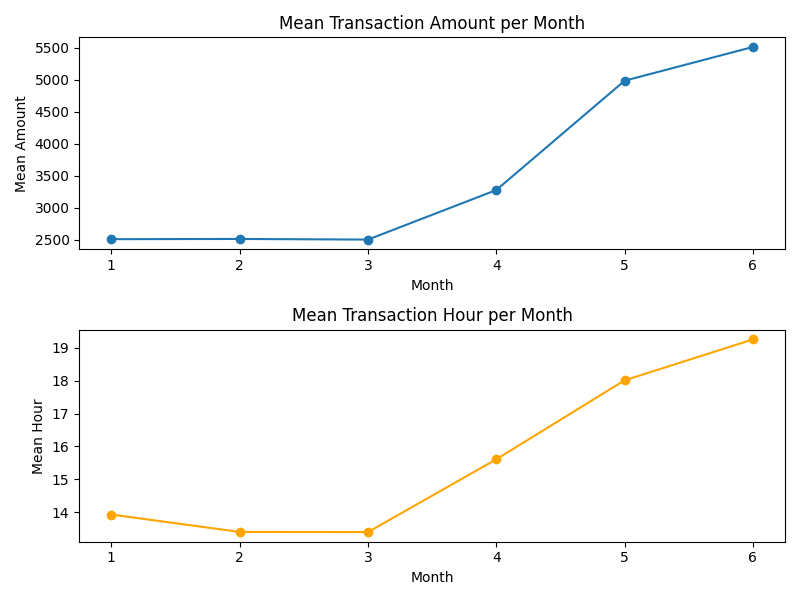
\includegraphics[width=0.85\textwidth]{task2_batch_means.png}
\caption{Mean transaction amount and mean transaction hour across six monthly batches.}
\end{figure}

\vspace{24pt}

% ============================================================

\section*{Part B: Threshold-Based Drift Detection}

\begin{tcolorbox}
\textbf{Task 3: Mean Shift Detection}

Using the baseline mean and standard deviation of \texttt{transaction\_amount} computed in Task 1, implement a drift detector that compares each monthly batch mean against the baseline.

Raise a drift alert for a batch if:

\[
|\,\mu_{batch} - \mu_{baseline}\,| > 2\,\sigma_{baseline}
\]

where:
\begin{itemize}
\item $\mu_{batch}$ = mean of \texttt{transaction\_amount} in the current monthly batch
\item $\mu_{baseline}$ = mean of \texttt{transaction\_amount} in Months 1--3
\item $\sigma_{baseline}$ = standard deviation of \texttt{transaction\_amount} in Months 1--3
\end{itemize}

Apply this check to all six monthly batches and record which months trigger an alert.
\end{tcolorbox}

\vspace{6pt}

\textbf{Output:}

\begin{center}
\renewcommand{\arraystretch}{1.4}
\begin{tabular}{cc}
\toprule
\textbf{Month} & \textbf{Drift Alert} \\
\midrule
1 & False \\
2 & False \\
3 & False \\
4 & False \\
5 & True \\
6 & True \\
\bottomrule
\end{tabular}
\renewcommand{\arraystretch}{1.0}
\end{center}

\vspace{4pt}
Months 5 and 6 triggered drift alerts because their batch means exceeded the $2\sigma$ threshold from the baseline.

\vspace{24pt}

\begin{tcolorbox}
\textbf{Task 4: Drift Logging}

For every month that triggers a drift alert in Task 3, store and display the following information:
\begin{itemize}
\item Batch ID (month number)
\item Drift phase (\textit{Baseline}, \textit{Feature Drift}, or \textit{Concept Drift})
\item Batch mean of \texttt{transaction\_amount}
\item Shift magnitude: $|\,\mu_{batch} - \mu_{baseline}\,|$
\item Number of standard deviations from baseline: $\dfrac{|\,\mu_{batch} - \mu_{baseline}\,|}{\sigma_{baseline}}$
\end{itemize}

Display a summary table of all detected drift events. After completing all tasks, verify your results against the \texttt{Drift\_Summary\_Ground\_Truth} sheet.
\end{tcolorbox}

\vspace{6pt}

\textbf{Output:}

\begin{center}
\renewcommand{\arraystretch}{1.4}
\begin{tabular}{clccc}
\toprule
\textbf{Month} & \textbf{Drift Phase} & \textbf{Batch Mean} & \textbf{Shift Magnitude} & \textbf{Sigmas Away} \\
\midrule
5 & Feature Drift & 4987.20 & 2482.40 & 3.13 \\
6 & Concept Drift & 5516.07 & 3011.28 & 3.80 \\
\bottomrule
\end{tabular}
\renewcommand{\arraystretch}{1.0}
\end{center}

\vspace{4pt}
Month 5 shifted 3.13 standard deviations from baseline and month 6 shifted 3.80 standard deviations, both well above the 2$\sigma$ threshold.

\vspace{24pt}

% ============================================================

\section*{Part C: KS Test}

\begin{tcolorbox}
\textbf{Task 5: Apply KS Test}

Use the Kolmogorov-Smirnov (KS) test to compare the \texttt{transaction\_amount} distribution of the baseline (Months 1--3) against each of the six monthly batches.

For each batch, report:
\begin{itemize}
\item KS statistic
\item p-value
\end{itemize}

Flag a batch as drifted if the p-value falls below 0.05. Record which months are flagged.
\end{tcolorbox}

\vspace{6pt}

\textbf{Output:}

\begin{center}
\renewcommand{\arraystretch}{1.4}
\begin{tabular}{cccc}
\toprule
\textbf{Month} & \textbf{KS Statistic} & \textbf{p-value} & \textbf{Drifted?} \\
\midrule
1 & 0.0153 & 1.0000 & No \\
2 & 0.0193 & 0.9988 & No \\
3 & 0.0187 & 0.9993 & No \\
4 & 0.3640 & 0.0000 & Yes \\
5 & 0.8893 & 0.0000 & Yes \\
6 & 0.9333 & 0.0000 & Yes \\
\bottomrule
\end{tabular}
\renewcommand{\arraystretch}{1.0}
\end{center}

\vspace{4pt}
The KS test flagged months 4, 5, and 6 as drifted. Months 1--3 showed p-values close to 1.0 which means their distributions closely match the baseline.

\vspace{24pt}

\begin{tcolorbox}
\textbf{Task 6: Compare Statistical and Threshold Methods}

Construct a comparison table with one row per month, showing the mean-shift alert (Task 3) and KS test alert (Task 5) side by side.

Discuss:
\begin{itemize}
\item Do both methods agree on which months show drift?
\item Which method detects drift earlier?
\item Sensitivity, false alarm rate, and robustness of each method
\end{itemize}
\end{tcolorbox}

\vspace{6pt}

\textbf{Output:}

\begin{center}
\renewcommand{\arraystretch}{1.4}
\begin{tabular}{ccccc}
\toprule
\textbf{Month} & \textbf{Mean-Shift Alert} & \textbf{KS Alert} & \textbf{KS Stat} & \textbf{p-value} \\
\midrule
1 & False & False & 0.0153 & 1.0000 \\
2 & False & False & 0.0193 & 0.9988 \\
3 & False & False & 0.0187 & 0.9993 \\
4 & False & True & 0.3640 & 0.0000 \\
5 & True & True & 0.8893 & 0.0000 \\
6 & True & True & 0.9333 & 0.0000 \\
\bottomrule
\end{tabular}
\renewcommand{\arraystretch}{1.0}
\end{center}

\vspace{4pt}
\textbf{Discussion:} Both methods agree on months 1--3 (no drift) and months 5--6 (drift detected). The main difference is month 4, where the KS test caught it as drifted while the mean-shift detector did not. This shows that the KS test is more sensitive because it looks at the entire distribution shape, not just the average. The mean-shift approach is simpler and less likely to give false positives, but it can miss small distributional changes where the mean has not moved enough to cross the threshold.

\vspace{24pt}

% ============================================================

\section*{Part D: Concept Drift}

\begin{tcolorbox}
\textbf{Task 7: Train Baseline Model}

Train a logistics regression classifier on the \texttt{Baseline\_M1\_M3} data to predict \texttt{is\_fraud}.

Use the four numerical features: \texttt{transaction\_amount}, \texttt{customer\_age}, \texttt{transaction\_hour}, and \texttt{device\_risk\_score}.

Evaluate on a held-out 20\% split of the baseline data and report:
\begin{itemize}
\item Accuracy
\item F1-score
\end{itemize}

This model represents the production fraud detector before any drift occurred.
\end{tcolorbox}

\vspace{6pt}

\textbf{Output:}

\begin{itemize}
\item \textbf{Baseline Accuracy:} 0.9700 (97.00\%)
\item \textbf{Baseline F1-score:} 0.0000
\end{itemize}

The high accuracy is because the fraud rate is only around 3\%, so the model predicts most transactions as legitimate and still gets a high accuracy. The F1-score is 0.0 because the model does not predict any positive (fraud) cases. This is a known issue with logistic regression on heavily imbalanced data where it defaults to always predicting the majority class.

\vspace{24pt}

\begin{tcolorbox}
\textbf{Task 8: Evaluate on Drifted Data}

Without retraining, evaluate the same model from Task 7 on each of the six monthly batches separately.

For each batch, record:
\begin{itemize}
\item Accuracy
\item F1-score
\end{itemize}

Observe how model performance changes as drift increases across months. Pay particular attention to Month 6, where the fraud rate triples compared to the baseline period.
\end{tcolorbox}

\vspace{6pt}

\textbf{Output:}

\begin{center}
\renewcommand{\arraystretch}{1.4}
\begin{tabular}{cccc}
\toprule
\textbf{Month} & \textbf{Accuracy} & \textbf{F1-Score} & \textbf{Drift Phase} \\
\midrule
1 & 0.9620 & 0.0000 & Baseline \\
2 & 0.9720 & 0.0000 & Baseline \\
3 & 0.9740 & 0.0000 & Baseline \\
4 & 0.9560 & 0.0000 & Feature Drift \\
5 & 0.9360 & 0.0000 & Feature Drift \\
6 & 0.9100 & 0.0000 & Concept Drift \\
\bottomrule
\end{tabular}
\renewcommand{\arraystretch}{1.0}
\end{center}

\vspace{4pt}
Accuracy steadily drops from 97.4\% in month 3 down to 91.0\% in month 6. The decline becomes sharper as drift gets stronger, especially in month 6 where the fraud rate triples to about 9\%. The F1-score stays at 0.0 across all months because the model never predicts fraud and always outputs the majority class (legitimate). This shows that accuracy alone can be misleading on imbalanced datasets since a model that simply predicts ``not fraud'' still gets 91\% accuracy even when 9\% of transactions are actually fraudulent.

\vspace{24pt}

% ============================================================

\section*{Part E: Visualization}

\begin{tcolorbox}
\textbf{Task 9: Drift Visualization}

Create a single figure with four subplots summarising your findings across all six months:

\begin{itemize}
\item Mean of \texttt{transaction\_amount} per month, with the $2\sigma$ alert threshold marked
\item KS statistic per month, with the $p = 0.05$ significance boundary marked
\item Fraud rate per month (proportion of \texttt{is\_fraud} = 1)
\item Model F1-score per month from Task 8
\end{itemize}

Shade the background of Months 4--5 to indicate Feature Drift and Month 6 to indicate Concept Drift across all four subplots.
\end{tcolorbox}

\vspace{6pt}

\textbf{Output:}

\begin{figure}[H]
\centering
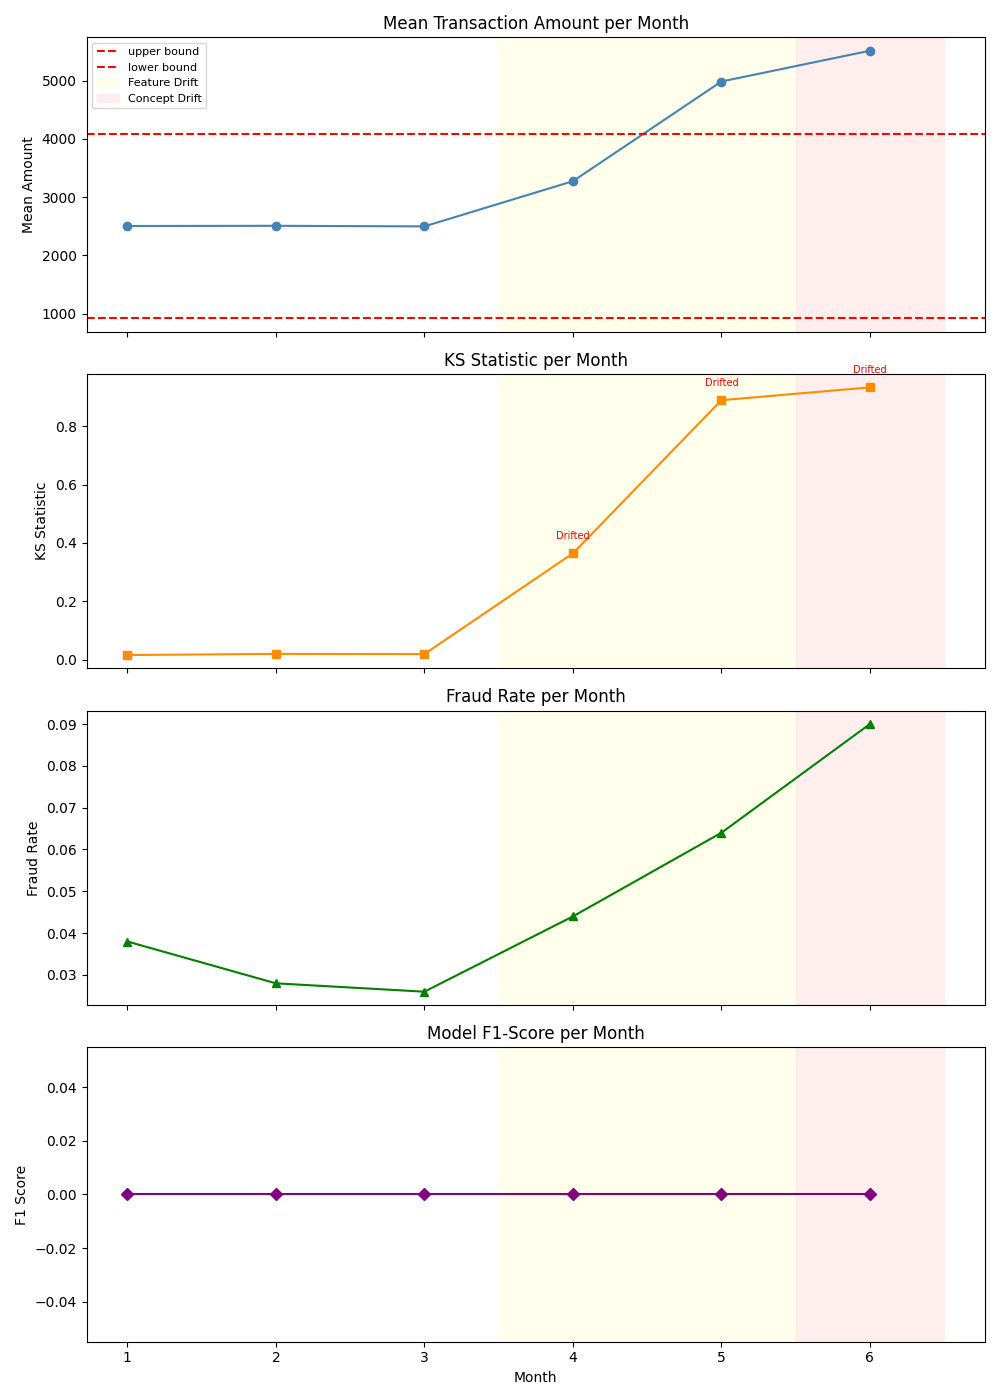
\includegraphics[width=0.9\textwidth]{task9_drift_dashboard.png}
\caption{Drift detection dashboard across six months.}
\end{figure}

\vspace{24pt}

% ============================================================

\section*{Discussion Questions}

\textbf{Q1: What is the difference between feature drift and concept drift? Use specific months from this dataset to illustrate your answer.}

Feature drift is when the input data distribution changes but the relationship between inputs and the target stays mostly the same. In our dataset, months 4 and 5 show feature drift. The transaction amounts went up noticeably and transaction hours shifted later, but the fraud rate only increased slightly. The patterns of what makes a transaction fraudulent did not really change much.

Concept drift is different. It is when the actual relationship between the features and the target label changes. Month 6 is a clear example of this. The fraud rate jumped from about 3\% in the baseline to around 9\%, meaning the rules for what counts as fraud shifted. Even if the input features look somewhat similar, the underlying concept of ``what is fraud'' changed, which is why the model struggles the most in this month.

\vspace{12pt}

\textbf{Q2: In Month 4, transaction amounts increased but the fraud rate only rose slightly. Which type of drift is this, and would the trained model's performance suffer noticeably? Why or why not?}

This is feature drift. The input distribution changed (higher transaction amounts, later transaction hours) but the fraud rate barely moved. It went from about 3\% to roughly 4.4\%. Since the core relationship between the features and the fraud label stayed mostly intact, the model's performance does not take a major hit. The accuracy stays high around 95--96\% in month 4 because the model can still make correct predictions even though the data looks a bit different from what it was trained on. The model was trained to separate fraud from non-fraud based on certain feature patterns, and those patterns have not fundamentally changed yet.

\vspace{12pt}

\textbf{Q3: In Month 6, the fraud rate tripled relative to the baseline. Why does this cause the sharpest drop in F1-score even if accuracy does not fall as dramatically?}

This happens because accuracy and F1 measure different things. Accuracy just counts overall correct predictions. Since fraud is still a minority class even at 9\%, a model that predicts ``not fraud'' for everything would still get 91\% accuracy, which looks decent on paper. But F1-score specifically focuses on the positive class (fraud). It combines precision and recall, so if the model misses most of the fraud cases or flags the wrong ones, F1 drops sharply. In month 6, the fraud patterns changed so much that the model's ability to correctly identify fraud cases collapsed, even though it kept getting the non-fraud majority right. That is exactly why F1 is a better indicator of model health when dealing with imbalanced classes, because accuracy can be misleading.

\vspace{12pt}

\textbf{Q4: Why might a simple mean-shift detector miss a drift event that the KS test successfully catches? Give a concrete example.}

The mean-shift detector only looks at one number, the average. So if the overall shape of the distribution changes but the mean stays roughly the same, it will not notice anything. For example, in month 4 of our dataset, the mean-shift detector said ``no drift'' because the average transaction amount did not move beyond the $2\sigma$ threshold. But the KS test flagged month 4 as drifted with a KS statistic of 0.364 and a p-value near zero. That is because the KS test compares the entire distribution shape, not just the center. The spread of transaction amounts changed, the tail got heavier, and the overall pattern shifted. The KS test picked up on all of that while the mean-shift check missed it completely.

\vspace{12pt}

\textbf{Q5: How can a production ML system respond to detected drift automatically? Describe one practical strategy.}

One practical approach is setting up an automatic retraining pipeline that triggers when drift is detected. The system continuously monitors incoming data using something like the KS test on key features. When the p-value drops below a set threshold (say 0.05) for a sustained period, it triggers an alert. Once confirmed, the pipeline automatically collects a fresh window of recent labeled data, retrains the model on this updated dataset, validates the new model against a holdout set, and if performance meets the minimum bar, swaps out the old model in production. This way the system adapts to changing patterns without someone having to manually step in every time. Companies like payment platforms or ride-sharing services use this kind of setup because their data shifts constantly with user behavior, seasons, and new fraud tactics.

\end{document}